\documentclass[conference,final]{IEEEtran}

\usepackage{latex8}
\usepackage{times}

\usepackage[utf8]{inputenc}
\usepackage{graphicx}
\usepackage{url}
\usepackage{float}
\usepackage{times}    
\usepackage{multirow}    
\usepackage{listings}   
\usepackage{times}     
\usepackage{paralist}    
\usepackage{wrapfig}    
\usepackage[small,it]{caption}
\usepackage{multirow}
\usepackage{ifpdf}


\usepackage{listings}
\usepackage{keyval}  
\usepackage{color}
\definecolor{listinggray}{gray}{0.95}
\definecolor{darkgray}{gray}{0.7}
\definecolor{commentgreen}{rgb}{0, 0.4, 0}
\definecolor{darkblue}{rgb}{0, 0, 0.4}
\definecolor{middleblue}{rgb}{0, 0, 0.7}
\definecolor{darkred}{rgb}{0.4, 0, 0}
\definecolor{brown}{rgb}{0.5, 0.5, 0}

\lstdefinestyle{myListing}{
  frame=single,   
  backgroundcolor=\color{listinggray},  
  %float=t,
  language=C,       
  basicstyle=\ttfamily \footnotesize,
  breakautoindent=true,
  breaklines=true
  tabsize=2,
  captionpos=b,  
  aboveskip=0em,
  belowskip=-2em,
  %numbers=left, 
  %numberstyle=\tiny
}      

\lstdefinestyle{myPythonListing}{
  frame=single,   
  backgroundcolor=\color{listinggray},  
  %float=t,
  language=Python,       
  basicstyle=\ttfamily \footnotesize,
  breakautoindent=true,
  breaklines=true
  tabsize=2,
  captionpos=b,  
  %numbers=left, 
  %numberstyle=\tiny
}

\newcommand{\up}{\vspace*{-1em}}
\newcommand{\upp}{\vspace*{-0.5em}}
\newcommand{\numrep}{8 }
\newcommand{\samplenum}{4 }
\newcommand{\tmax}{$T_{max}$ }
\newcommand{\tc}{$T_{C}$ }
\newcommand{\bj}{BigJob}

\title{Running Bio-ensemble Simulations on Azure and Hybrid, Heterogeneous Cloud Infrastructures}

\author{
Andr\'e Luckow$^{1}$, Shantenu Jha$^{1,2,3,*}$,\\
  \small{\emph{$^{1}$Center for Computation \& Technology, Louisiana State University, USA}}\\
  \small{\emph{$^{2}$Department of Computer Science, Louisiana State University, USA}}\\
  \small{\emph{$^{3}$e-Science Institute, Edinburgh, UK}}\\
  \small{\emph{$^{*}$Contact Author: \texttt{sjha@cct.lsu.edu}}}\\
}

%\date{}

\def\acknowledgementname{Acknowledgements}
\newenvironment{acknowledgement}%
{\section*{\acknowledgementname}%
\parindent=0pt%
}

\newif\ifdraft
%\drafttrue
\ifdraft
\newcommand{\llnote}[1]{ {\textcolor{green} { ***JK: #1 }}}
\newcommand{\alnote}[1]{ {\textcolor{blue} { ***AL: #1 }}}
\newcommand{\jhanote}[1]{ {\textcolor{red} { ***SJ: #1 }}}
\else
\newcommand{\llnote}[1]{}
\newcommand{\alnote}[1]{}
\newcommand{\jhanote}[1]{}
\fi

\begin{document} 

\maketitle    

\begin{abstract}
  
\end{abstract}

\section{Introduction}

Scope:
\begin{itemize}
    \item Running Bio-ensembles on Azure and hybrid Grid/Clouds
    \item Amazon Cluster Compute benchmark
\end{itemize}


\section{SAGA and SAGA-based Frameworks for Large-Scale and
  Distributed Computation} 

SAGA~\cite{saga_url} provides a simple, POSIX-style API to the most
common Grid functions at a sufficiently high-level of abstraction so
as to be independent of the diverse and dynamic Grid environments. The
SAGA specification defines interfaces for the most common
Grid-programming functions grouped as a set of functional packages
(Fig.~\ref{Fig:SAGA1}). Some key packages are:

\begin{figure}[!ht]
 \begin{center}
     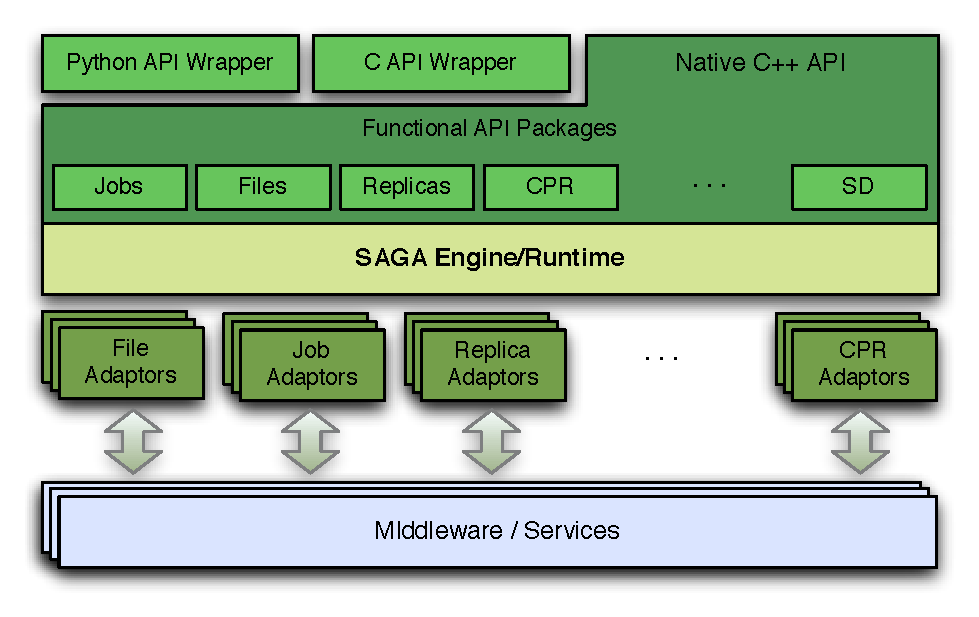
\includegraphics[width=0.45\textwidth]{figures/stci_saga_figures-1.pdf}
 \end{center}
\caption{\small Layered schematic of the different components of the
   SAGA landscape. At the topmost level is the simple integrated API
   which provides the basic functionality for distributed
   computing. Our BigJob abstraction is built upon this SAGA layer
   using Python API bindings.\up} \label{Fig:SAGA1}
\end{figure}

\begin{itemize}
\item File package - provides methods for accessing local and remote
 filesystems, browsing directories, moving, copying, and deleting
 files, setting access permissions, as well as zero-copy reading and
 writing.
\item Job package - provides methods for describing, submitting,
 monitoring, and controlling local and remote jobs. Many parts of
 this package were derived from the largely adopted
 DRMAA specification. 
% ~\cite{drmaa_url} 
\item Other Packages, such as the RPC (remote procedure call), Replica
  package and Stream Package.  
  % remote socket connections with hooks to
  %   support authorization and encryption schemes.
\end{itemize}

In the absence of a formal theoretical taxonomy of distributed
applications, Fig.~\ref{Fig:sagaapps} can act a guide.  Using this
classification system, there are three types of distributed
applications: (i) Applications where local functionality is swapped
for distributed functionality, or where distributed execution modes
are provided.  A simple but illustrative example is %an ensemble of
an application that uses distributed resources for bulk
submission. Here, the application remains unchanged and even unaware
of its distributed execution, and the staging, coordination, and
management are done by external tools or agents. Most applications in
this category are classified as implicitly distributed.  (ii)
Applications that are naturally decomposable or have multiple
components are then aggregated or coordinated by some unifying or
explicit mechanism.  DAG-based workflows are probably the most common
example of applications in this category.  Finally, (iii) applications
that are developed using frameworks, where a framework is a generic
name for a development tool that supports specific application
characteristics (e.g. hierarchical job submission), and recurring
patterns (e.g. MapReduce, data parallelism) and system functionality.
Lazarus~\cite{enkf-gmac09} provides several autonomic features, such as
fault tolerance and dynamic resource selection, specifically for 
Ensemble-Kalman-Filter application scenarios.
SAGA has been used to develop system-level tools and applications for
each of these types.



\begin{figure}[!ht]
  \begin{center}
    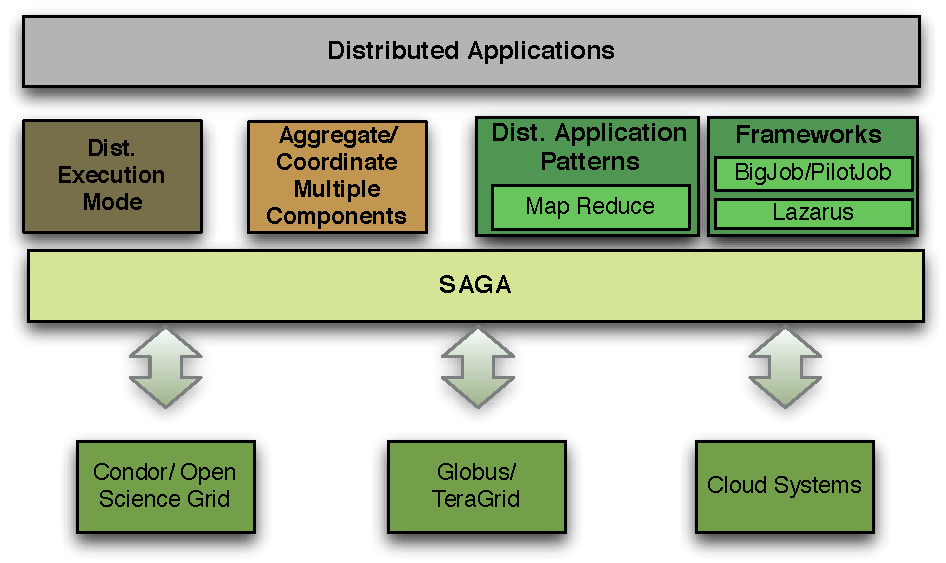
\includegraphics[width=0.45\textwidth]{figures/distributed_applications_saga_figure.pdf}
  \end{center}
  \caption{\small Showing the ways in which SAGA can be used to
    develop distributed applications.  The different shaded box
    represent the three different types; frameworks in turn can
    capture either common patterns or common application
    requirements/characteristics. \label{Fig:sagaapps} \up}
\end{figure}

It is important to note that SAGA provides the basic API to implement
distributed functionality required by applications (typically used
directly by the first category of applications), and is also used to
implement higher-level APIs, abstractions, and frameworks that, in
turn, support the development, deployment and execution of distributed
applications~\cite{enkf-gmac09}. Merzky et\,al.~\cite{sagamontage09} 
discusses how SAGA was used to implement a higher-level API to support
workflows. In this paper, we will discuss how SAGA can be used to
implement runtime frameworks to support the efficient execution of the
distributed applications.

\section{Windows Azure}

Azure provides different higher level services, e.\,g.\ the Azure
AppFabric or Azure Storage, that can be accessed via HTTP/REST from
anywhere. Windows Azure offers a platform for on-demand computing and
for hosting generic server-side applications. The so-called Azure
fabric controller automatically monitors alls VMs, automatically
reacts to hardware and software failures and manages application
upgrades.

\subsubsection{Compute}
Windows Azure formalizes different types of virtual machines into
so called roles. Web roles e.\,g.\ are used to host web applications
and frontend code, while worker roles are well suited for background
processing. While these roles target specific scenarios, they are also
highly customizable. Worker roles can e.\,g.\ run native code. The
application must solely implemented a defined entry point, which is
then called by Azure. The Azure fabric controller automatically
manages and monitors applications, handles hardware and software
failures as well as updates to the operating system or to the
application.  Commonly, scientific applications utilize worker roles
for compute- and data-intensive tasks. AzureBlast~\cite{azure_blast}
e.\,g.\ heavily relies on worker roles for computing bio-sequences.

\subsubsection{Storage}
For storing large amounts of data the Azure storage platform
provides three key services: the \emph{Azure Blob Storage} for storing
large objects of raw data, the \emph{Azure Table Storage} for
semi-structured data and the \emph{Azure Queue Storage} for
implementing message queues.  The data is storage replicated across
multiple data centers to protect it against hardware and software
failures. In contrast to other cloud offerings (e.\,g.\ Amazon S3) the
Azure Storage Services provide strong consistency guarantees, i.\,e.\
all changes are immediately visible to all future calls. While
eventual consistency as implemented by S3~\cite{1294281} usually
offers a better performance and scalability, it has some disadvantages
mainly caused by the fact that the complexity is moved to the
application space.

The blob storage can store file up to a size of 1\,TB, which makes it
particularly well suited for data-intensive application. The Amazon S3
service e.\,g.\ restricts the maximum file size to 5\,GB. Further, the
access to the blob storage can be optimized for certain usage modes:
\emph{block blob} can be split into chunks which can be uploaded and
downloaded separately and in parallel.  Thus, block blobs are well
suited for uploading and streaming large amounts of data. \emph{Page
  blob} manage the storage as an array of pages. Each of these pages
can be addressed individually, which makes page blobs a good tool for
random read/write scenarios. \emph{Azure XDrive} provides a durable
NTFS volume, which is backed by a page blob. In particular legacy
applications that heavily utilize file-based storage can simply be
ported to Azure using XDrive.

The Azure Queue Service provides a reliable storage for the delivery
of messages within distributed applications.  The queue service is
ideal to orchestrate the various components of a distributed
applications, e.\,g.\ by distributing work packages or collecting
results, which could be running on Azure or on another resource,
e.\,g.\ a science cloud.

The Azure Table Storage is ideally suited for storing structured
data. Unlike traditional relational database systems, the table
storage is designed with respect to scale-out, low cost and high
performance similar to Google's BigTable~\cite{bigtable2006}
system. For legacy application Azure also provides a SQL-Server based,
relational datastores called SQL Azure. In contrast to Azure tables,
SQL storage supports common relation database features, such as
foreign keys, joins and SQL as query language.


\section{BigJob: SAGA-based Pilot-Job Framework}
%\up

%\jhanote{do we want \emph for bigjob?} \alnote{yes,looks good for introducing the term.}
\emph{BigJob} is a SAGA-based Pilot-Job implementation. In contrast to
other Pilot-Job implementations, e.g., Falkon, BigJob natively
supports parallel applications (e.g. based on MPI) and works
independent of the underlying Grid infrastructure across different
heterogeneous backend, e.\,g.\ Grids and Cloud, reflecting the
advantage of using a SAGA-based approach. Further, the framework is
extensible and provides several hooks that can be used to support
other resource types and Pilot-Job frameworks.
% \jhanote{We have talked about interoperability; need to address extensibility} 
% \alnote{Added sentence before}

As shown in Figure~\ref{fig:figures_distributed_pilot_job}, BigJob currently
provides a unified abstraction to Grids, Condor pools and
Clouds. Using the same API, applications can dynamically allocate
resources via the big-job interface and bind sub-jobs to these
resources. In the next sections, we describe how SAGA interfaces to
three different backends, while exposing the same user-level BigJob interface
and semantics. A tutorial that describes the BigJob API can be found 
at~\cite{bigjob_cloud_tutorial}.

% \jhanote{Should the second level in the upperbox be ``SAGA BigJob
%   API''?}\alnote{changed}
%\up
\begin{figure}[htbp]
    \centering
        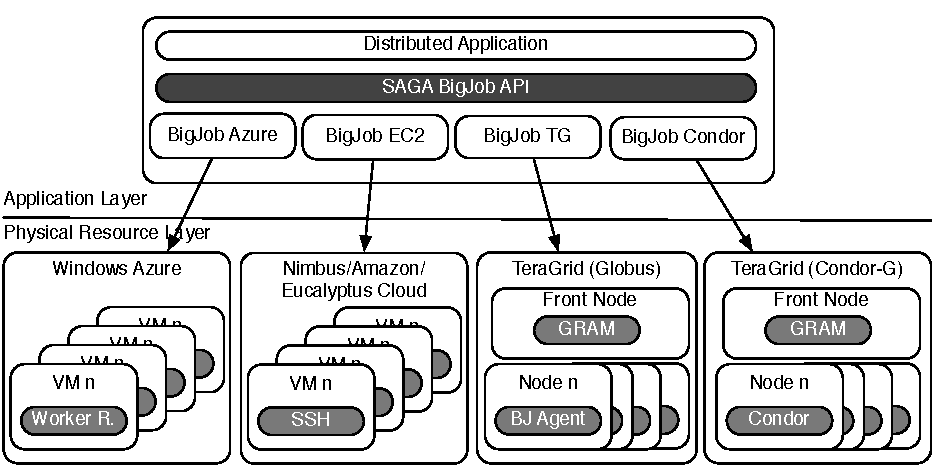
\includegraphics[width=0.45\textwidth]{figures/distributed_pilot_job}
        \caption{\textbf{Overview of the SAGA-based Pilot Job:} The
          SAGA Pilot Job API is currently implemented by three
          different backends - one for Grids, Condor and for
          Clouds.\up}
    \label{fig:figures_distributed_pilot_job}
\end{figure}




\subsection{BigJob for Grids}
\up

Figure~\ref{fig:figures_bigjob} shows an overview of the SAGA BigJob
implementation for computational Grids. The Grid BigJob comprises of
three components: (i) the BigJob Manager that provides the Pilot-Job
abstraction and manages the orchestration and scheduling of BigJobs
(which in turn allows the management of both big-job objects and
sub-jobs), (ii) the BigJob Agent that represents the pilot job
\jhanote{Can we use something other than pilot job} and thus, the
application-level resource manager on the respective resource, and
(iii) advert service which is used for communication between the
BigJob Manager and Agent.


\begin{figure}[ht]
    \centering
    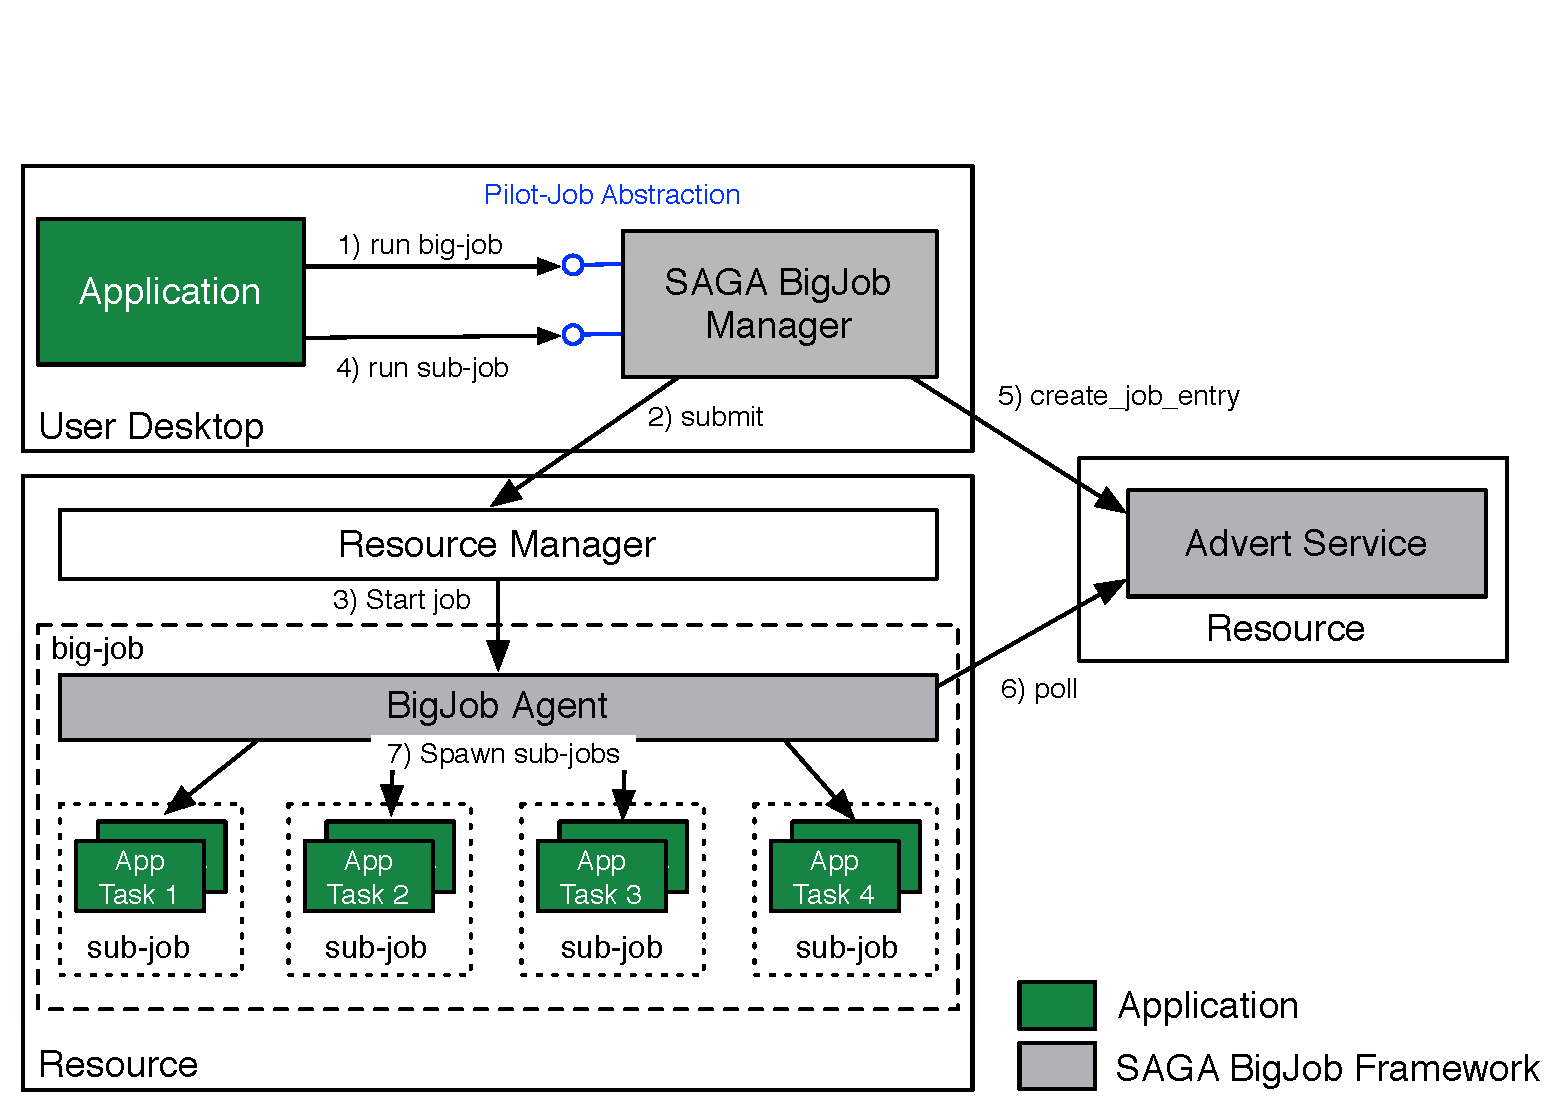
\includegraphics[width=0.45\textwidth]{figures/bigjob}
   \caption{BigJob Architecture: The core of the framework, the
      BigJob Manager, orchestrates a set of sub-jobs via a
      BigJob Agent using the SAGA job and file APIs.  The
      BigJob Agent is responsible for managing and monitoring sub-jobs.\up}
   \label{fig:figures_bigjob}
\end{figure}

Applications can utilize the framework via the big-job and sub-job
classes. Both interfaces are syntactically and semantically consistent
with the other SAGA APIs: a sub-job e.\,g.\ is described using 
the standard SAGA job description; job states are expressed
using the SAGA state model. Before running sub-jobs, an application must initialize
a big-job object. The BigJob Manager then queues a job,
% \jhanote{are we confusing the reader by toggling between Pilot-Job
%   and BigJob?} \alnote{ok, change to Grid job}
which actually runs a BigJob Agent on the respective remote
resource. For this agent a specified number of resources is
requested. Subsequently, sub-jobs can be submitted through the BigJob
Manager using the job-id of the BigJob as reference. The BigJob
Manager ensures that sub-jobs are launched onto the correct
resource based upon the specified job-id using the right number of
processes. 

The Grid BigJob is a SAGA-based framework and heavily utilizes the
SAGA job, file and advert APIs. The BigJob Agent is started using the
SAGA job API.  Communication between the BigJob Agent and BigJob
Manager is carried out using the SAGA advert service, a central
key/value store. For each new job, an advert entry is created by the
BigJob Manager. The agent periodically polls for new jobs. If a new
job is found and resources are available, the job is dispatched,
otherwise it is queued.

% \jhanote{But mention that this work is different in that, (i) it
%   establishes the general principles and design, and is used for a
%   range of applications, (ii) extends capabilities to work with
%   Clouds, and (iii) sets the stage for extensible Pilot-Job
%   functionality, e.g., policy-driven pilot-jobs.  Need to mention the
%   general purpose nature: both HTC and HTC of HPC, as well that it is
%   more than just a container of ensemble based applications.  It
%   provides the framework for deploying and supporting
%   application-level runtime environments.}

In this paper we will use BigJob to support HPC applications, however,
BigJob has also been used to support high-throughput runs of HPC
applications on the TeraGrid. Specifically, 
El-Khamra et\,al.~\cite{enkf-gmac09} uses BigJob to support a very
large number of ensembles with highly variable run-times, as well as
heterogenous resource requirements.  In Luckow et\,al.~\cite{repex_ptrs}
although an efficient scale-out behaviour was established, all resources
utilized were TeraGrid resources, and thus accessible using a uniform
Globus interface. Another use cases that have used BigJob on Grid
resources include applications involving parameter sweeps and which
require the execution of a very large number of simulations in
parallel.  Having outlined the general principles and design
objectives of the BigJob framework, and established its use on
production grid infrastructure for a range of applications, we will
focus on extending its capabilities to work with Clouds and other
distributed infrastructure.




\subsection{BigJob for Azure}
\up
% espite a standardized interface, big difference on how to obtain meta-data (internal ip etc.)

Figure~\ref{fig:figures_bigjob_azure} illustrates the architecture of the BigJob
for Azure building blocks. The BigJob Manager (BM) is responsible for accepting 
simulation requests from the end-user and for orchestrating the sub-job runs. 
In the future these capabilities can be extended by supporting more advanced steering and
visualization features. The BM creates work packages for each sub-job and 
distributes them via the Azure Queue Service and
later collects the results stored by the replicas in the Azure
storage.  The BigJob Agents run within Azure worker roles, which are
ideally suited for running background tasks. Azure enables users to
run native code within worker roles, i.\,e.\ the framework will be
able to support numerous MD codes, e.\,g.\ NAMD~\cite{Phillips:2005gd}
and AMBER~\cite{cheatham-5}.  Azure currently does not support MPI
computations across multiple worker roles, thus each MD
simulation is limited to 8 cores.



%\begin{wrapfigure}{R}{0.4\textwidth}
\begin{figure}
    \centering
    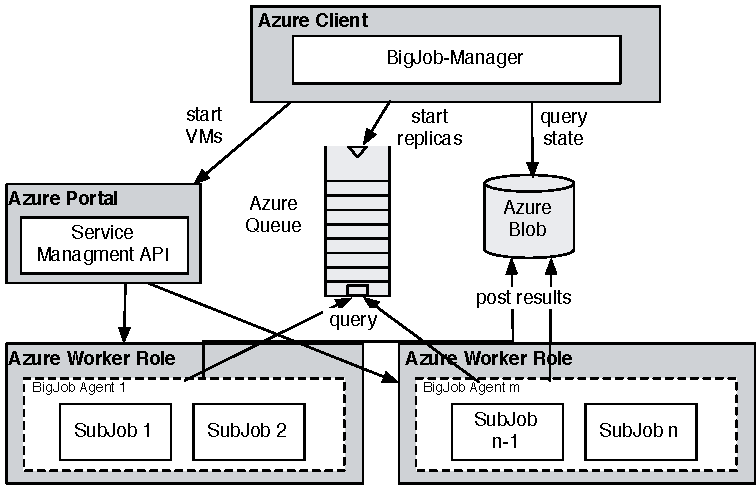
\includegraphics[width=.4\textwidth]{figures/bigjob_azure}
    \caption{\textbf{Azure-based BigJob:} The framework
      utilizes the queue storage for distributing work
      packages from the BigJob Manager to the
      BigJob agents running on multiple worker roles.}
    \label{fig:figures_bigjob_azure}
\end{figure}


The worker roles running the replica agent are managed by the RM using
the Azure Service Management API. In the initial version we will
support the automatic start and stop of hosted services. In the final
version there will be a possibility to automatically deploy agent code
without the need to pre-configuring the VMs. Once the agents are
started, they query the Azure queue for new work items. If a work item
is found, a simulation task is started, e.\,g.\ by running the requested
MD code with right parameters.  The number of
MD jobs per worker role depends on the size of the worker role --
Azure currently supports worker roles up to 8 cores.

% \alnote{Kalman Filter option: we need to convey how we make decisions?
% we need to understand the various trade-offs}

The ensemble use case can greatly benefit from the
capabilities of Azure. If greater accuracy is required or a deadline
must be met, it can seamlessly scale-out to more worker roles.  The
Azure fabric controller monitors all VMs running the worker roles and
automatically restarts the worker roles if necessary. Further, Azure
provides various kinds of reliable and scalable storage options to
express different coordination schemes, e.\,g.\ the master-worker
communication can be conducted via the described message queue.


\section{Usage Modes and Analysis}

The aim of this section is not to perform detailed systematic
performance measures and analysis, but to illustrate the
representative usage modes BigJob can support, and to explain how they
are supported.  We discuss two scenarios that are representative of
how applications would typically use multiple distributed
infrastructures. We focus our attention on replica-based Molecular Dynamics (MD)
simulations and a workload as \numrep replicas of a Hepatatis-C virus
(HCV) model, each replica running for 500 timesteps.  


\section{Conclusion and Future Directions}



\begin{acknowledgement} 
  \up \footnotesize{Important funding for SAGA has been provided by
    the UK EPSRC grant number GR/D0766171/1 (via OMII-UK) and HPCOPS
    NSF-OCI 0710874. SJ acknowledges the e-Science Institute,
    Edinburgh for supporting the research theme, ``Distributed
    Programming Abstractions'' and theme members for shaping many
    important ideas. This work has also been made possible thanks to
    the internal resources of the Center for Computation \& Technology
    at Louisiana State University and computer resources provided by
    LONI. We thank Yaakoub El Khamra for help with initial experiments
    with the Condor infrastructure. We thank Joohyun Kim (CCT) for
    assistance with the RNA models. We thank FutureGrid and
    ScienceCloud for Nimbus resources.}
\end{acknowledgement}

\up
\bibliographystyle{IEEEtran}
\bibliography{literatur,saga,cloud}
\end{document}



